\section{Components}

\subsection{Chip-Card}
We use simple memory cards with $I^2$C-Bus and form factor ID-00 as specifyed in ISO 7816. They are quite cheap (less then 1\euro{} per Card) and are not secure. Their contents might be easily read or modifyed. So everyone can read and check what we write on their card.

%-----

\subsection{realtimeclock (RTC)}
The realtimeclock is implemented in software by using one of the microcontrollers timers. A timerinterrupt function increments a 64bit value every millisecond (this counter will wrap arround in about 584.542.046 years, which should be quite enough for us). Additionaly the counters value is periodically\footnote{the value is backed up every $3FFFFF_{(16)}$ milliseconds wich is about every 1.165 hours} written to the microcontrollers eeprom and read back after reset. On reset we also add the value $3FFFFF_{(16)}$ to the counter to avoid having more then on time the same timestamp.

\subsection{random number generator (RNG)}
\begin{window}[0,r, 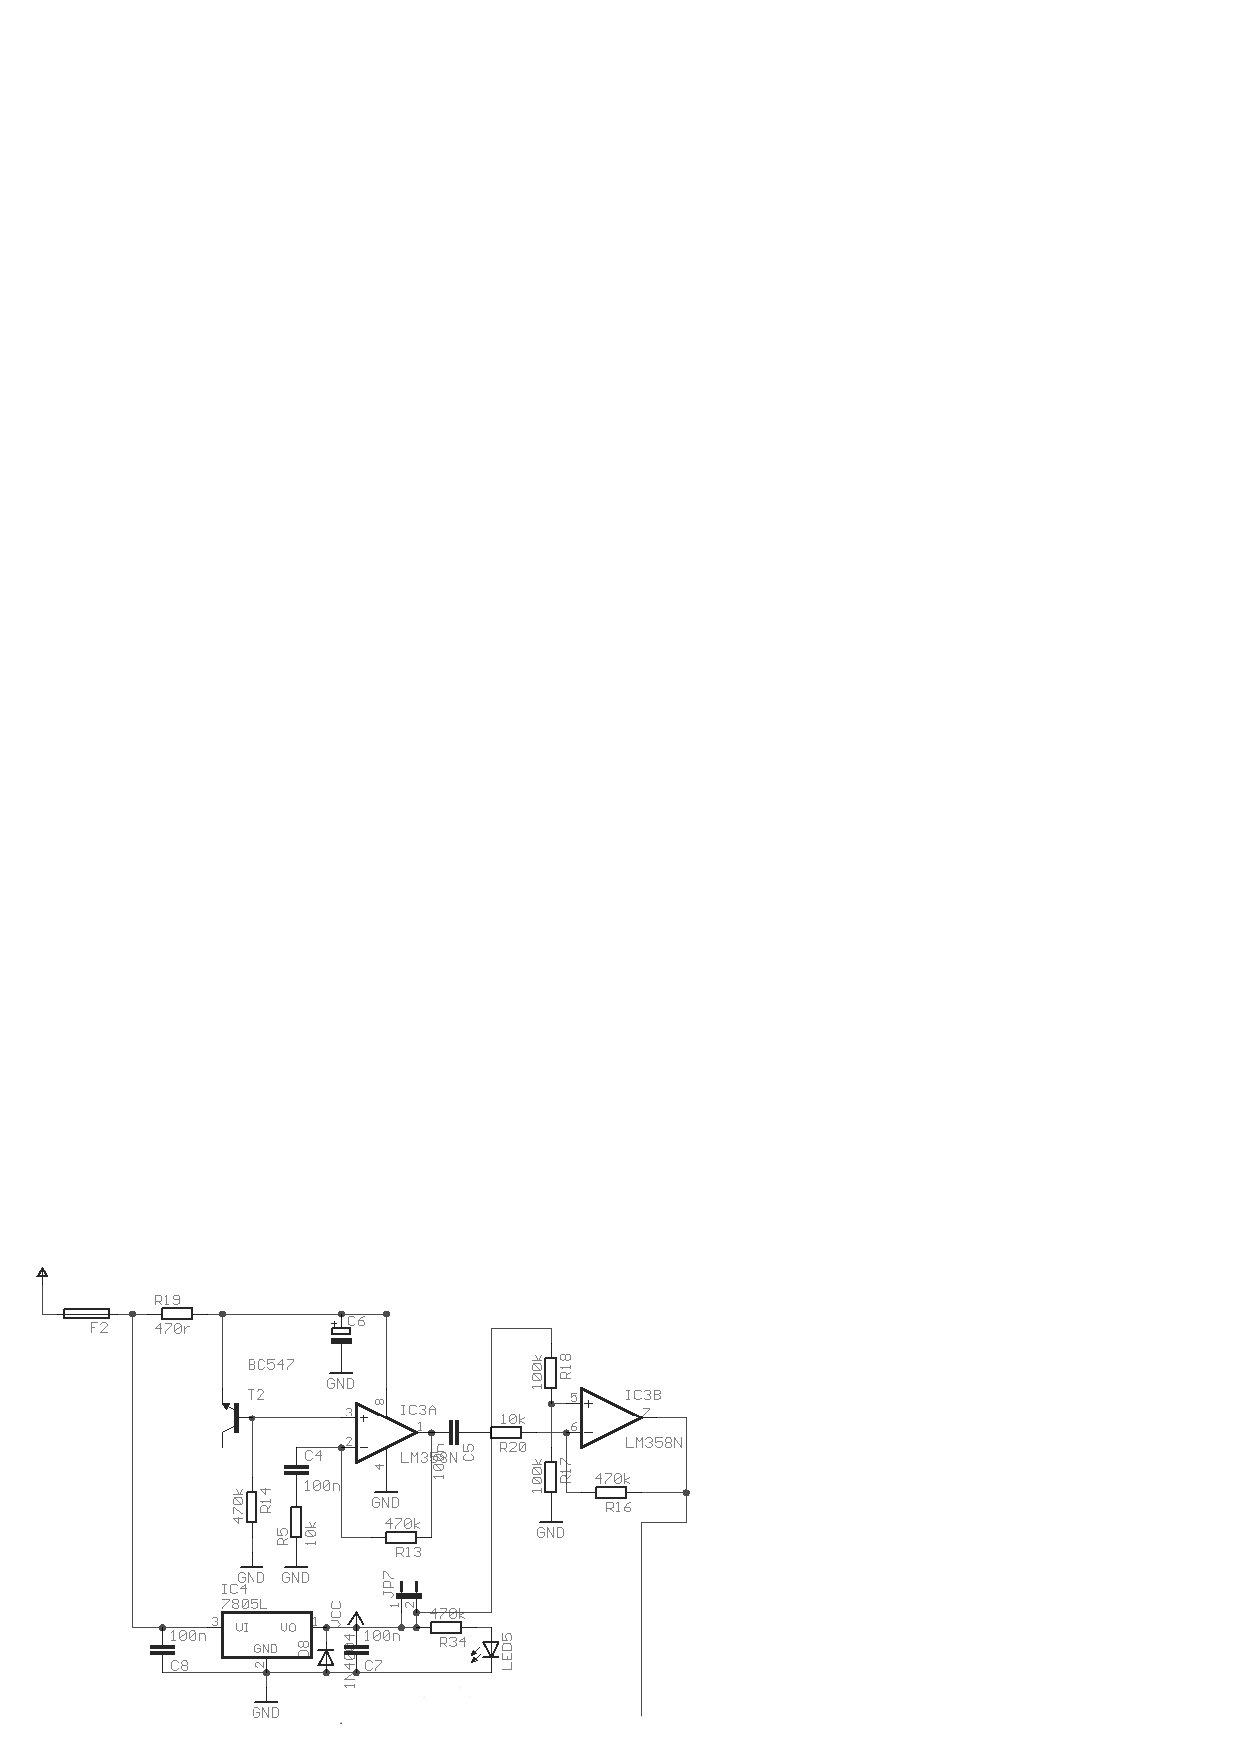
\includegraphics[scale=0.5]{RNG}, {schematic of the hardware random generator}]
This curcit utilises the randomnes of the breakthrough voltage of the diode of a transistor to generate random voltages in the range from 0 to 5 volts. While this is quite random it does not need to be cryptographicaly secure because the RNGs output is used only as input for the cryptograpicaly secure PRNG. \\
\{bla, bla, bla, bla, bla, bla, bla, bla, bla, bla, bla, bla, bla, bla, bla, bla, bla, bla, bla, bla, \}
\end{window}
%-----

\subsection{pseudornadom number generator (PRNG)}
The PRNG is based on the SHA-256 hash function and is specified in Appendix A.
It has two main functions:
\begin{itemize}
 \item AddEntropy: this function adds data to the entropy pool, the input can be of arbitary bit length
 \item GetRandomBlock: this function fills a 32 byte block of memory with a randomised bitstring
\end{itemize}
An other function (GetRandomByte) uses a buffer and the GetRandomBlock function and returns a random byte.
The PRNG is periodicaly filled with entropy from the hardware RNG using the AddEntropy function.
%-----

\subsection{secure serial port (QPort-tiny)}

%-----

\subsection{external serial eeprom}
The external serial eeprom is used to keep the two databases and can be used for key-exporting for migration. We use standard $I^2C$ EEPROMs with 512Kbit or 1Mbit (24xx512 or 24xx1025) from Microchip. It is possible to extend the storage capabilitys by using multiple EEPROMs. This makes it possible to have up to 4Mbit or 512Kbytes of storage space wich normally allows more than 10.000 users.

The whole contents of the eeprom is encrypted (except the keymigration-area). Shabea-16 is used to encrypt the content. We therfore divide the eeprom space into 32 byte blocks which are encrypted seperatly. Every block is encrypted with an individual key which is the result of concatenation of the ''main-key'' and the blockaddress. So we are protected against most attacs against massstorage-encryption (ex. watermarking) 

%-----

\subsection{Ticket-Database (TicketDB)}
This database is used to store a HMAC of the users ticket, her/his permissions, and some statistics about the whole system.
The first element in the database is the header followe by the entrys for the users.\\
\begin{tabular}{|l|c|l|}\hline 
name & size & description \\ \hline
ID & 10 bytes & set to the string ''AnonAccess'' \\
majversion & 1 byte & majorversion; set to 1 \\
minversion & 1 byte & minorversion; set to 0 \\
headersize & 1 byte & specifies the size of the header \\
stat & 10 bytes & statistics \\
reserved & 8 bytes & reserved field for future extensions and for alignement; set to 0 \\ \hline
\end{tabular} 


 the statistics field has the following structure:\\
\begin{tabular}{|l|c|l|} \hline
name & size & description \\ \hline 
max\_users     & 2 bytes & maximum number of users \\
users              & 2 bytes & actualy active user \\
admins           & 2 bytes & actualy active admins \\
locked\_users   & 2 bytes & number of locked users \\
locked\_admins & 2 bytes & number of locked admins \\ \hline
\end{tabular} 

The following space of the ticketDB is filled with userentrys which have the following structure:\\
\begin{tabular}{|l|c|l|} \hline
name & size & description \\ \hline 
flags         & 1 byte    & the flags associated with the user \\
nickname  & 7 bytess & the nickname if the user decided to be known by name \\
ticketmac  & 32 bytes & HMAC from users ticket \\ \hline
\end{tabular} 

Where the flag field has the following structure: \\
\begin{tabular}{|l|c|l|} \hline
name & size & description \\ \hline 
exists         & 1 bit    &  indicates if this entry is used (1: in use; 0: free)\\
admin  & 1 bit & set if user has admin privileges, cleared othewise \\
locked  & 1 bit & set if user is locke; cleared otherwise \\
noitfy\_lostadmin  & 1 bit & set if user has to be notifyed about lost admin privileges \\
anonymous  & 1 bit & set if the user did not specify username to be stored \\
reserved & 3 bit & reserved, should be set to 0\\ \hline
\end{tabular} 


%-----

\subsection{FlackModifying-Database (FLMDB)}




